\chapter{System Level Description}

\section{Master-Slave Pairing}

The whole FPGA system development circles around this fundamental idea of Masters and slave peripherals. The slave peripheral needs to be in
the memory map of the Master peripheral so that the master can access it by making memory requests on the interconnect. The below figure
shows a 1 Master - 1 Slave configuration with an interconnect IP interfacing them. As is visible the interconnect needs both the clocks on which
the peripherals operate in order to interface them by employing dual clocking FIFOs for each AXI channel.

\begin{figure}[H]
\centering
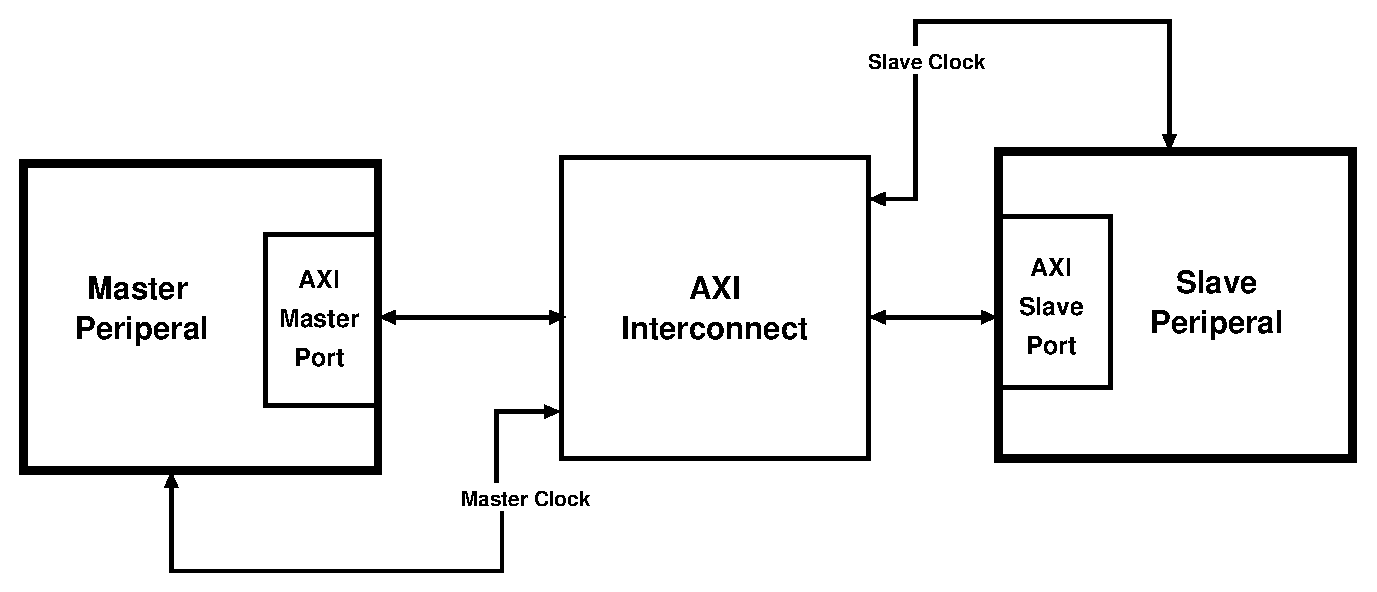
\includegraphics[width=\textwidth]{eps_pdf_sources/ajit_fpga/System_Level/One_Master_One_Slave}
\caption{1 AXI Master - 1 AXI Slave Configuration}
\end{figure}

The AXI Interconnect which bind the whole system is a NoC ( Network on Chip ) implementation of the communication subsystem and hence brings
notable improvements over conventional bus and crossbar communication architectures. Networks-on-chip improve the scalability of
systems-on-chip and the power efficiency of complex SoCs compared to other communication subsystem designs. 

\begin{figure}[H]
\centering
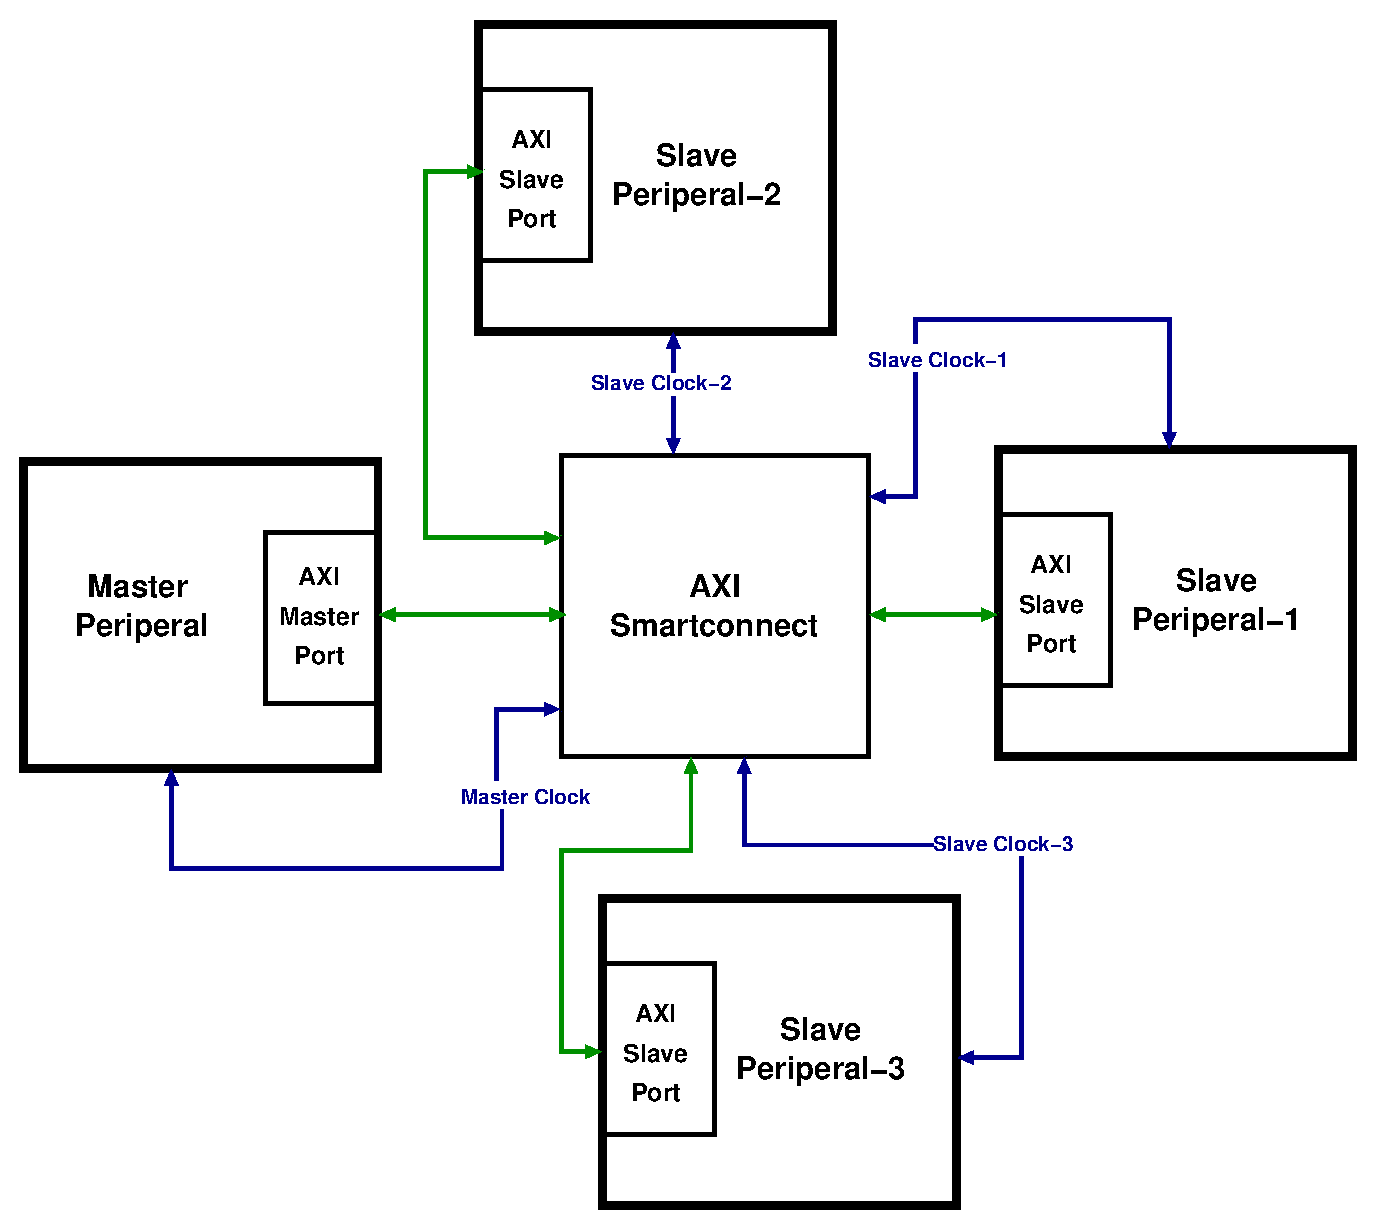
\includegraphics[width=\textwidth]{eps_pdf_sources/ajit_fpga/System_Level/One_Master_Multi_Slave}
\caption{1 AXI Master - 3 AXI Slave Configuration}
\end{figure}

\section{Dual Clocking FIFOs in Interconnects}

Dual clock FIFOs are designed for two circuits operating in different clock frequencies to communicate with each other. There is a read side
and write side where data is stored into the internal memory of the FIFO using the write side clock and then read from the internal memory
using the read side clock. AXI Smartconnect IPs from Xilinx employ dual clocking FIFOs to interface Master and slaves which have operate at
different clock frequencies for example AJIT core operates at 100MHz but the PCIe-AXI Translation IP operates at 250MHz thus we need
something like an AXI Smartconnect which can handle this interfacing situation.\\

\section{Memory mapped devices}

This age old approach is a regular practice on desktop, portable and embedded devices. This makes a device registers appear like a memory
location which can be manipulated with userspace applications.This makes writing to AXI peripherals through AJIT really convenient, the
reading and writing just becomes writing to the device file \verb|\dev\mem| on the AJIT Linux OS, this will initiate the appropriate memory
request from the AJIT core to the AXI interconnect through the AFB-AXI Bridge to the on board DRAM.

\section{Peripheral Control Interface}

The AXI Slave interface for each peripheral on the AXI Interconnect has some data registers and some control registers which include start
idle, and done bits. The start bit is written high after writing the data to the appropriate data registers and then the status bit i.e. the
done bit can be polled continuously until the peripheral is found to be done with the task. This is obviously a cumbersome process but works
out just fine for less number of peripherals, as the system matures we would need the peripherals to raise an interrupt to the processor
core whenever it is finished with the assigned task or if some error has occurred while execution of the task. 

\section{Processor as a peripheral} 

The AJIT processor wrapper has been designed so to have 2 AXI slave interfaces for debugging and 1 AXI Master interface for memory reads and writes
which are done indirectly through the AFB-AXI bridge as explained later. The below figure shows the wrapping done around in order to make it
in raw sense AXI interfaceable. As you can see inside the wrapper, AJIT resides in the center and right adjacent to it on the right is the
AFB-AXI Bridge which has been explained in detail later but for time being can be understood just as a bridge between the custom data bus of
AJIT i.e. AFB and the AXI interface. To the left of AJIT core are 2 64 bit FIFOs which are supposed to carry the 64 bit number sent from the
host which contains debug commands. To even further left of these FIFOs are their controllers which provide an AXI interface control of
these FIFOs to the masters on interconnect which includes the host machine(more on this later). These in combination provide AJIT
processor an interface ability to the AXI interface and makes AJIT core just another AXI Master peripheral on the AXI interconnect.\\

\begin{figure}[H]
\centering
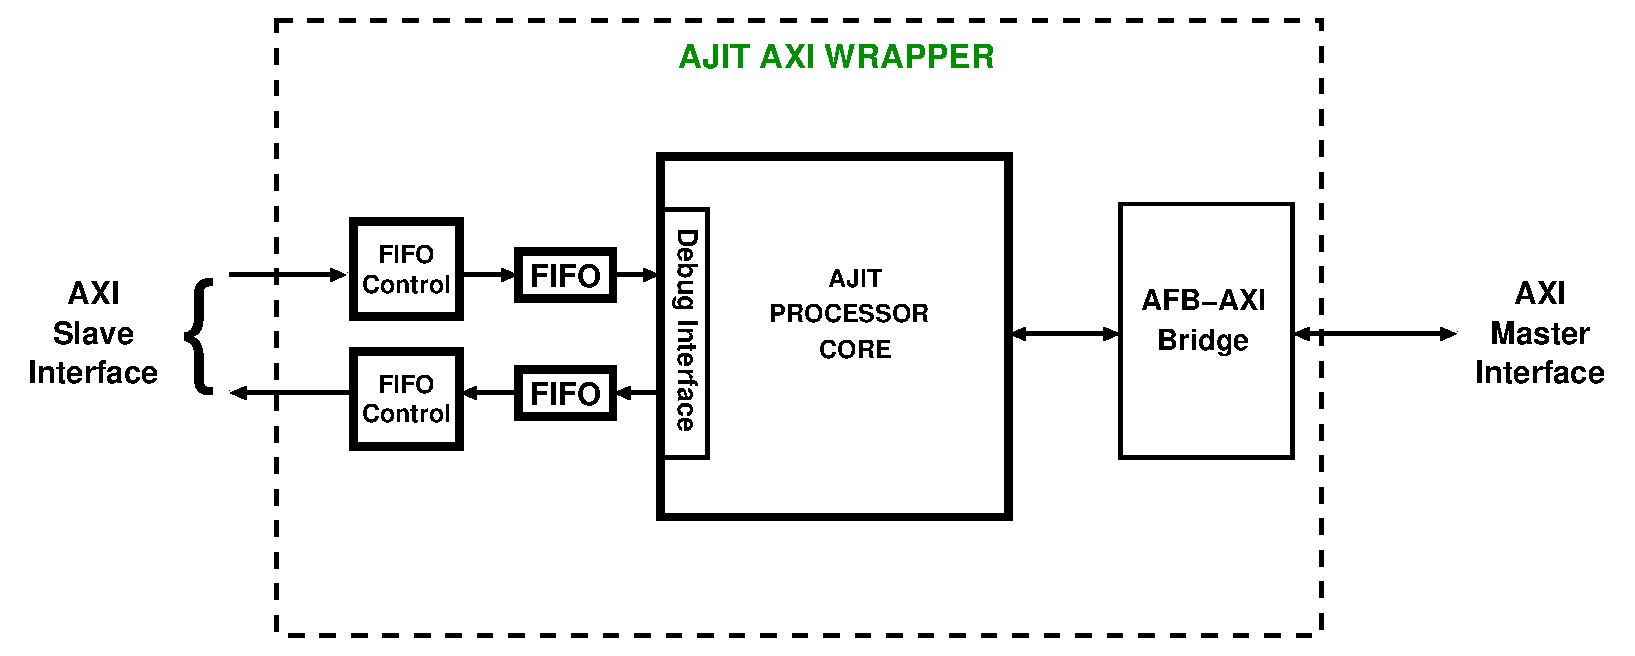
\includegraphics[scale=0.6]{eps_pdf_sources/ajit_fpga/System_Level/ajit_combined}
\caption{AJIT AXI Wrapper}
\label{ajit_combined}
\end{figure}

